
\newcommand{\PaperTitleOne}{Paper One's Title}

\section{\PaperTitleOne}

\begin{flushright}
Author 1, Author 2, Author 3
\end{flushright}

This feature includes a PDF file directly into the compiled LaTeX document.

See the \href{http://www.ctan.org/tex-archive/macros/latex/contrib/pdfpages/}{pdfpages}
package documentation.

The following pages are from the direct inclusion of the file
\textbf{pdf/paper\_one.pdf}.

Note that the table of content of the included pdf must be manually set in \break
\textbf{pdf\_include\_section.tex}.

Also, a .pax file was generated by \textbf{pdfannotextractor} on the (to be
included) \textbf{pdf/paper\_one.pdf}. This allows \textit{pdflatex} to include
all hyperlinks from the original PDF in the new one.
See \url{http://www.ctan.org/tex-archive/macros/latex/contrib/pax/}. Pax is
normally provided by TeXlive on linux (extra/texlive-latexextra on ArchLinux).

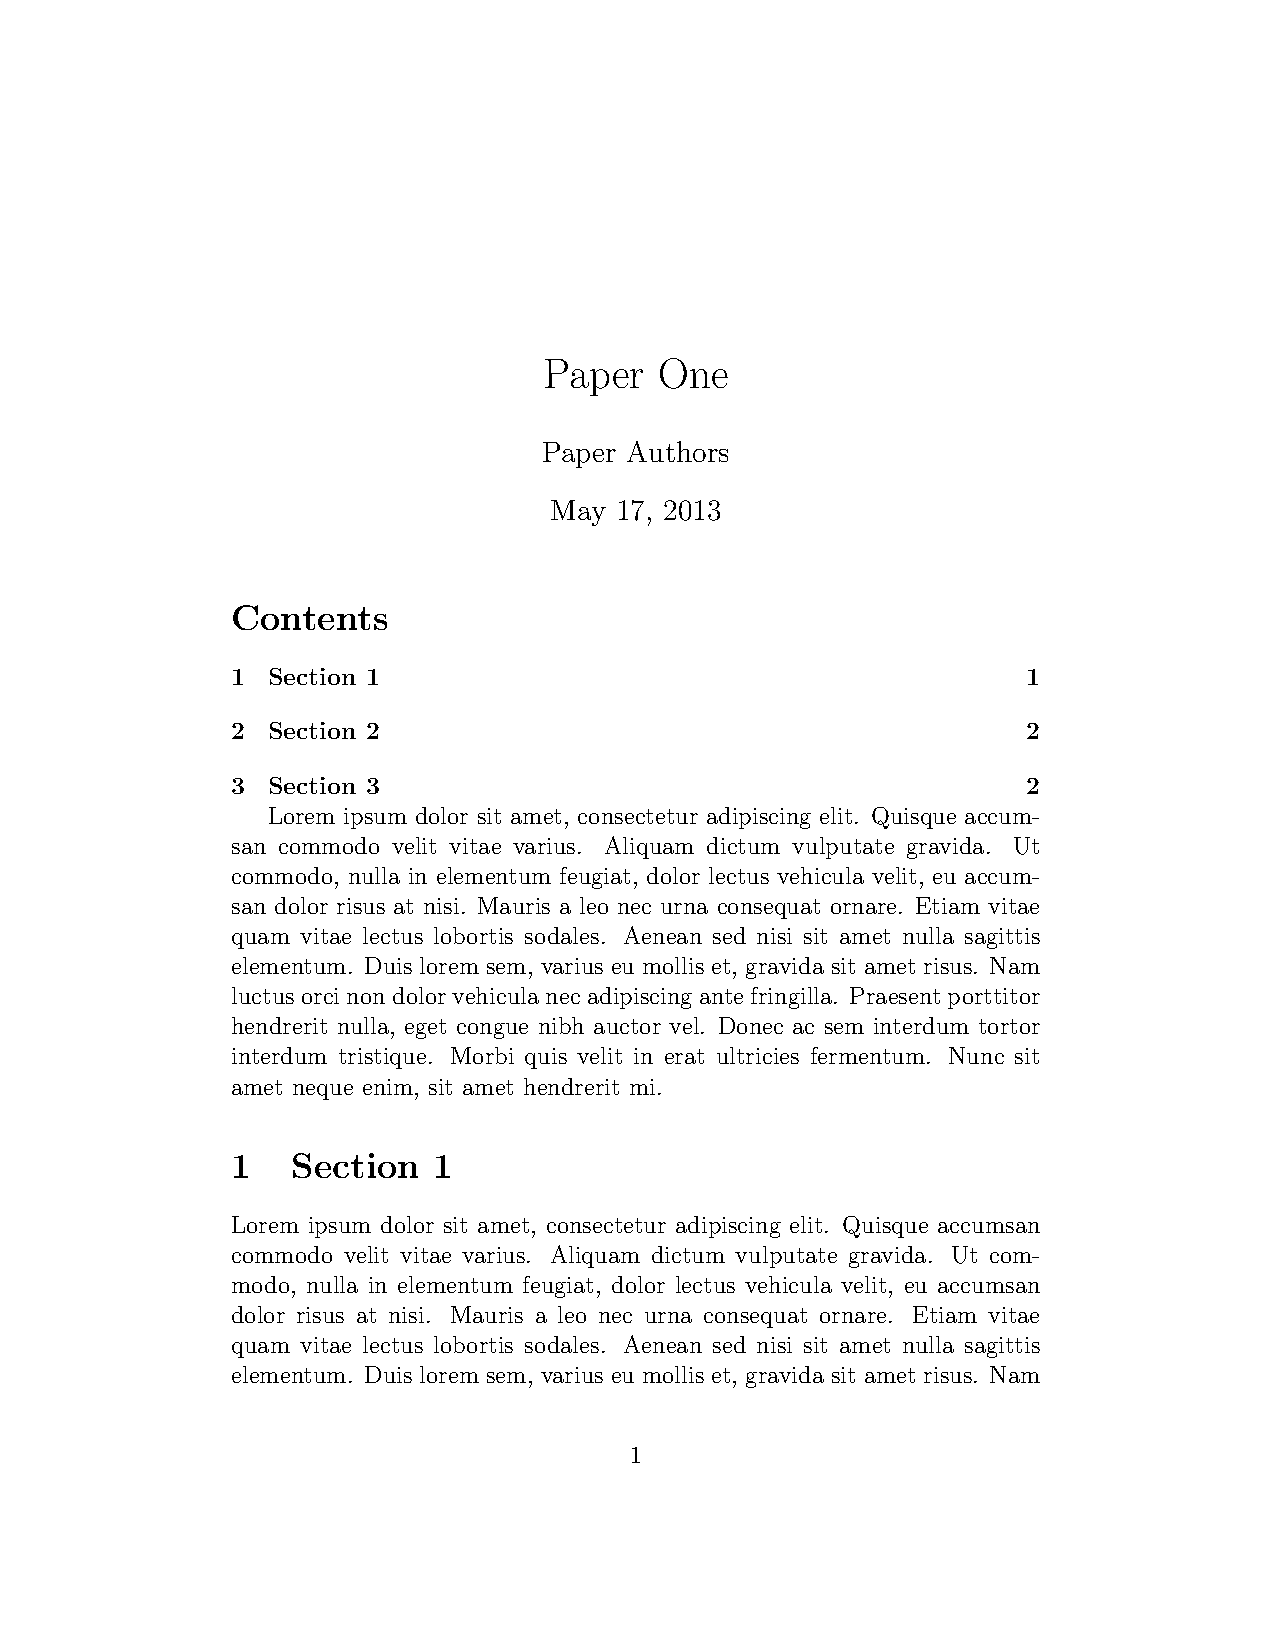
\includepdf[pages=-,
            addtotoc={
                1,subsection,2,Title Page,paper_one_title,
                1,subsection,2,Content,paper_one_content,
                1,subsection,2,Section 1,paper_one_section_one,
                2,subsection,2,Section 2,paper_one_section_two,
                2,subsection,2,Section 3,paper_one_section_three
            }]{pdf/paper_one.pdf}
